
\chapter{Trabajos relacionados}
\label{sec:chapter2}

En este cap\'itulo se muestran los trabajos relacionados al proyecto propuesto
 en este documento y una breve descripci\'on de estos, se podr\'a observar una
 diferencia tem\'atica entre la tem\'atica de los trabajos mostrados; empezando 
 por aquellos que tienen por objetivo ayudara a los discapacitados, 
 posteriormente los trabajos cuyo objetivo es que un robot mec\'anico o virtual 
 realice tareas de manera similar a como las har\'ia un ser humano y finalmente 
 se muestran m\'etodos para trabajar con datos categ\'oricos, de manera m\'as 
 espec\'ifica, datos nominales, ya que se contempla desarrollar un clasificador 
 no supervisado de datos nominales.
 

\section{Antecedentes}

%/***************************************************************************/

Desde el Microsoft Windows $3.11$ \cite{RomeroZunica1998} hasta la actualidad las 
 Opciones de accesibilidad de Microsoft Windows han permitido que el
 sistema operativo sea posible usarlo sin importar las condiciones f\'isicas del
 usuario \cite{DanielHubbell2016}. A continuaci\'on, se menciona una breve 
 descripci\'on de estas opciones.

\begin{itemize}
	\item Lupa: Aumenta el tama\~no del contenido de la pantalla para que sea
	 m\'as f\'acil leerlo \cite{xatakaaccesiblilidad}.
	\item Narrador:  Esta funci\'on es una ayuda auditiva que ayuda a saber 
	 cu\'ales son las ventanas abiertas y su contenido, por medio de una voz
	 sintetizada \cite{xatakaaccesiblilidad}.
	\item Teclado en pantalla: Como su nombre lo indica es un teclado virtual
	 con el cual podemos escribir presionando la pantalla, en caso de ser un
	 dispositivo t\'actil, o presionando los botones con el rat\'on
	 \cite{xatakaaccesiblilidad}.
	\item Contraste alto: Otra ayuda visual para poder distinguir mejor los
	 elementos en pantalla modificando el contraste de Windows
	 \cite{xatakaaccesiblilidad}.
	\item Reconocimiento de voz: Es una herramienta de dictado con la cual
	 se puede escribir y manipular aplicaciones e incluso el mismo sistema
	 operativo por medio de comandos de voz \cite{support14213}.
\end{itemize}

Aunque no esta considerado dentro de las opciones de accesibilidad de Windows,
 el asistente \emph{Microsoft Cortana} facilita la realizaci\'on de algunas tareas por medio de
 comandos de voz, por ejemplo, apertura de programas, la manipulaci\'on de
 recordatorios, mensajes de texto y correo electr\'onico \cite{support17214}. 


Los archivos por lotes (Batch o Script Shell) \cite{Silberschatz1999} son
 aquellos que contienen instrucciones para el sistema operativo en formato
 ASCII por lo que son dependientes de \'el, por lo general tienen la extensi\'on
 .bat o .sh, sin embargo, para el caso de UNIX esto no es obligatorio. En la
 figura~\ref{fig:script} se muestra el c\'odigo de un archivo por lotes y la 
 ejecuci\'on en consola.



\begin{figure}[h]
\centering
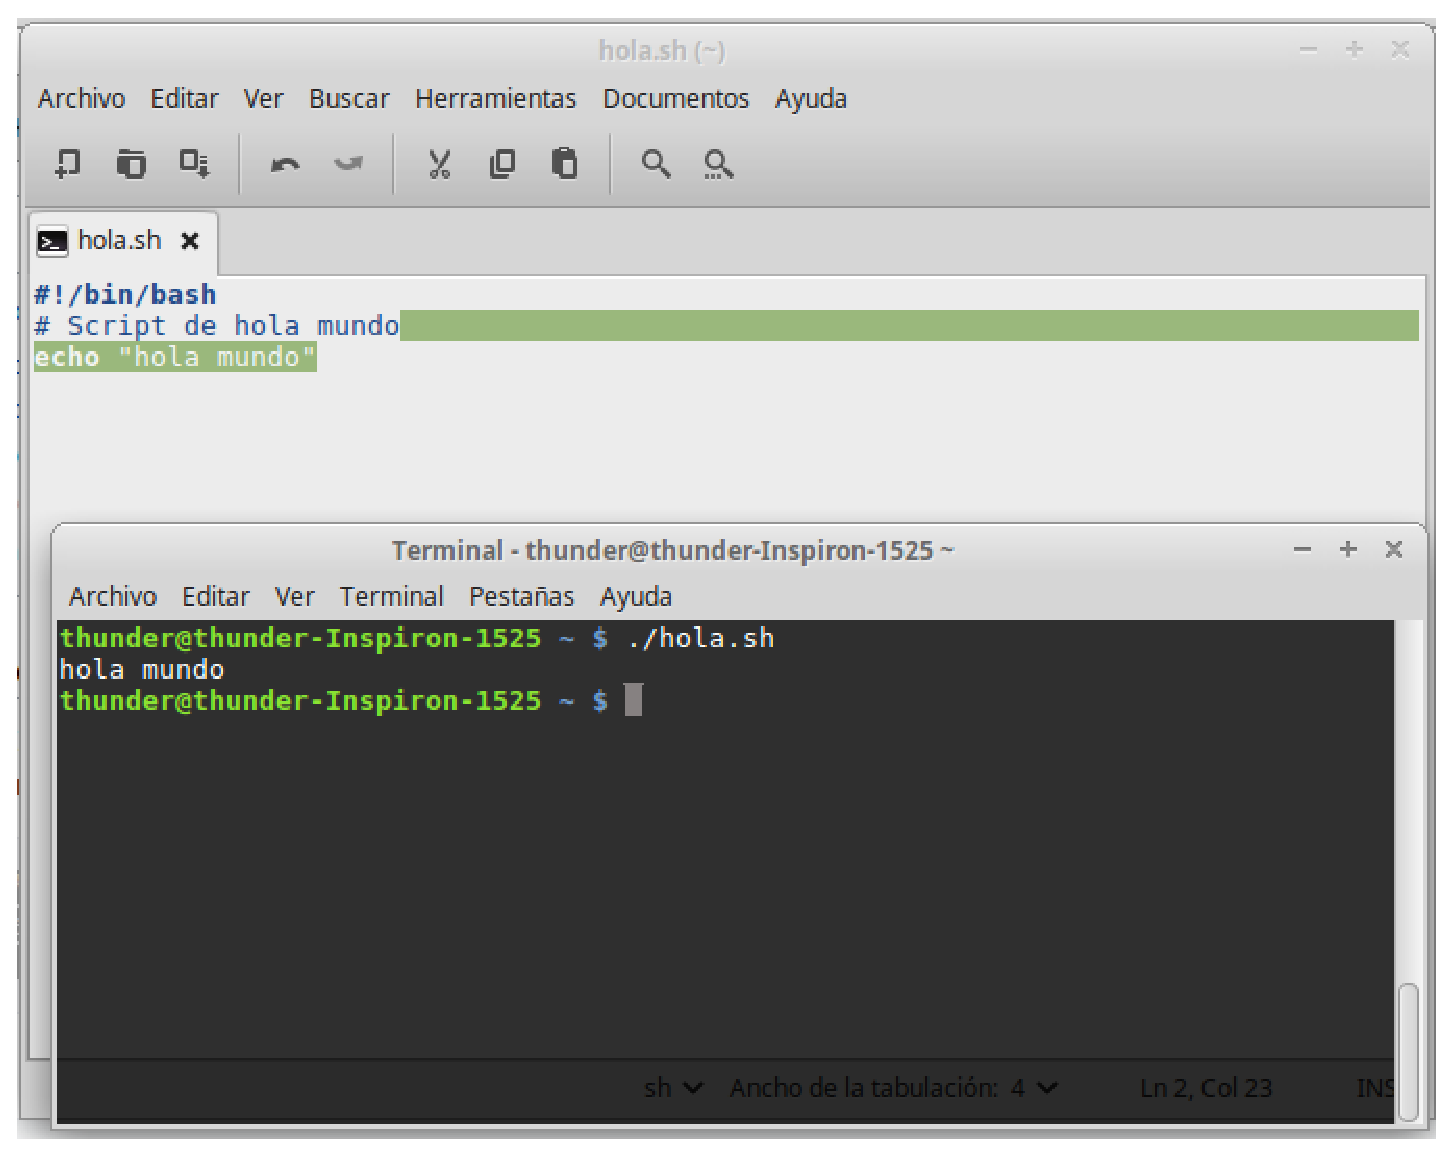
\includegraphics[width=0.7\columnwidth]{chap2/Imagenes/Script.eps}
\caption{Ejecuci\'on de un archivo por lotes en Linux.}
\label{fig:script}
\end{figure}

Pulover\textsc{\char13}s Macro Creator\cite{Batista}, desarrollado y mantenido
 principalmente por Rodolfo U. Batista, es una herramienta de automatizaci\'on
 y creaci\'on de scripts basada en el lenguaje ``AutoHotKey''. Este creador de
 macros facilita la tarea de la creaci\'on del script por medio de su interfaz
 gr\'afica \'o con la grabadora de macros que proporciona. Entre sus
 caracter\'isticas destaca el proporcionar control de ventanas en segundo plano
 y sentencias de control(ciclos y condicionales). En la figura
 ~\ref{fig:macros} se puede observar la interfaz de usuario del software.


\begin{figure}[h]
\centering
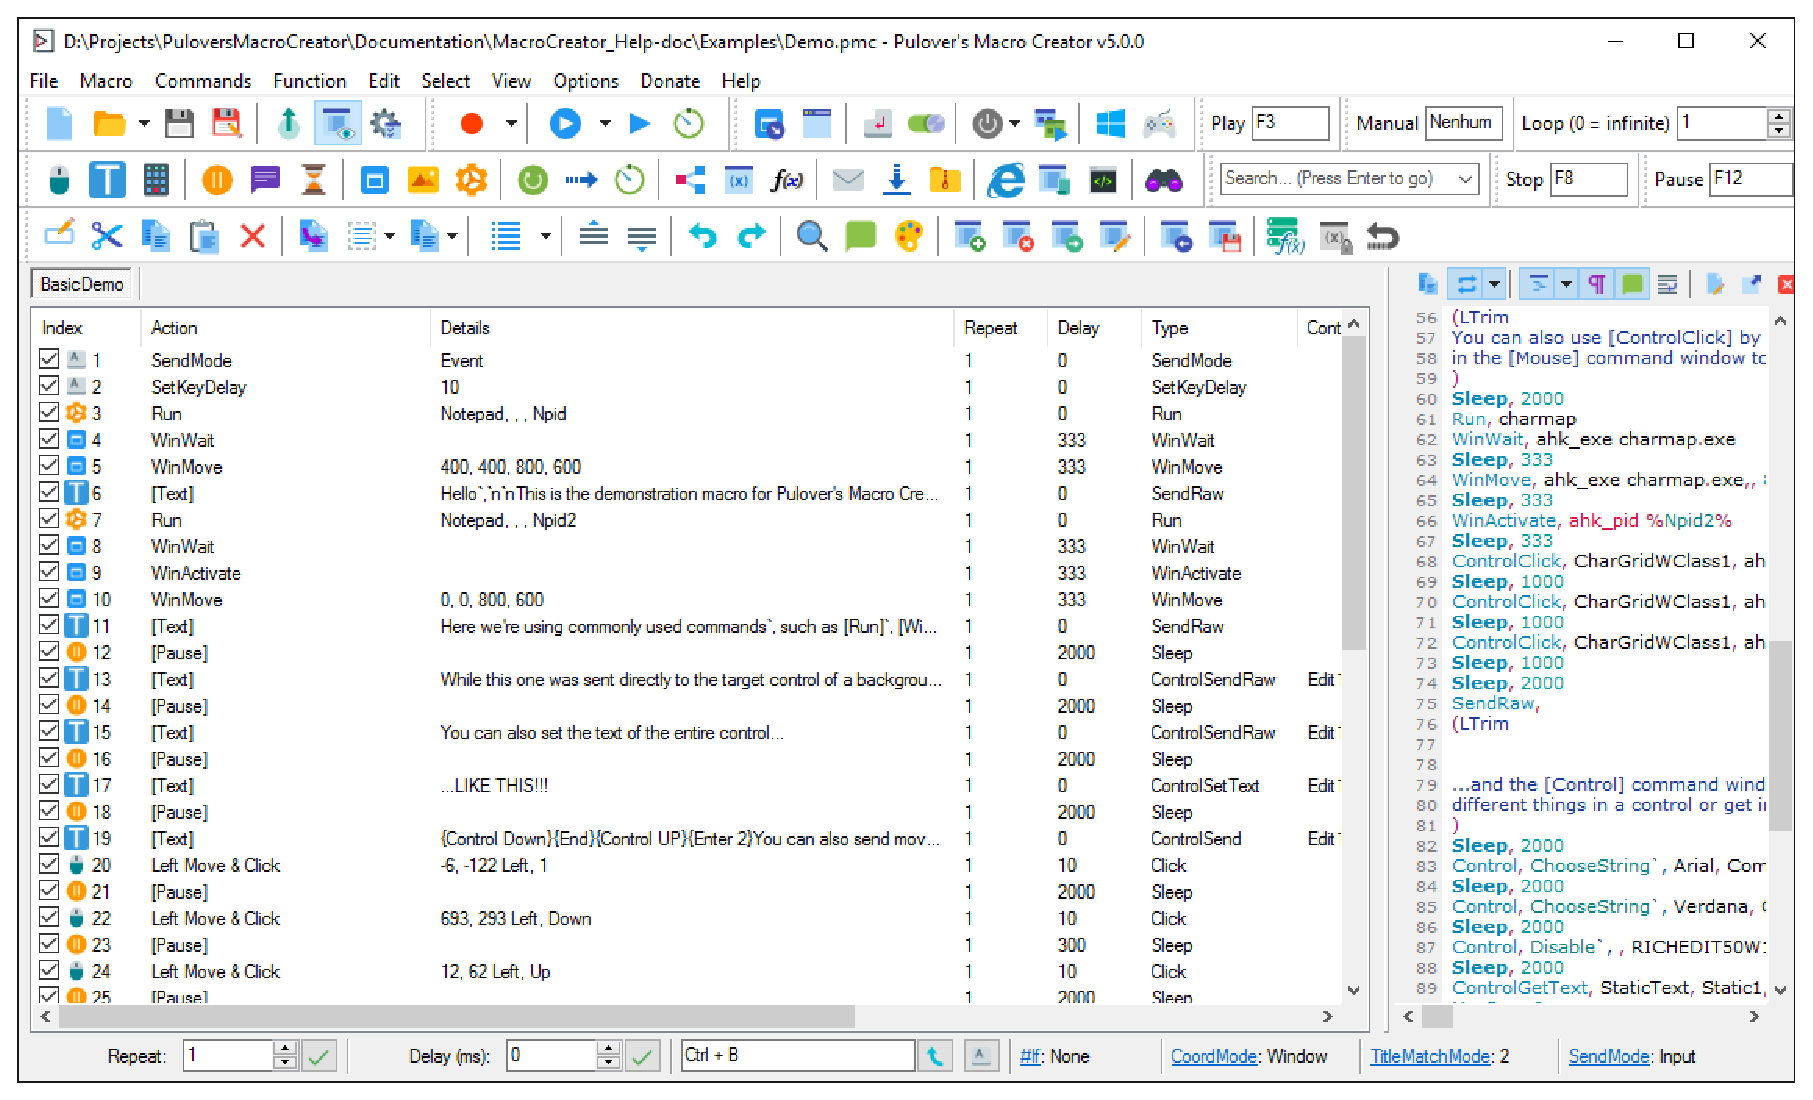
\includegraphics[width=0.7\columnwidth]{chap2/Imagenes/Macros.eps}
\caption{Interfaz de usuario de Pulovers Macro Creator con una macro de
 ejemplo proporcionada por el desarrollador\cite{Batista}.}
\label{fig:macros}
\end{figure}

\section{Estado actual de la ciencia}


Un trabajo desarrollado por la Universidad de Tsukuba en
 Jap\'on\cite{Nakano2006}, tiene por objetivo el crear un oponente virtual
 al nivel de un oponente humano que represente un reto para el jugador. Para
 lograr esto se crearon perfiles con las estrategias de los jugadores y
 posteriormente se reproducen en otra partida, en la figura~\ref{fig:imitat}
 se muestra el entorno del juego.


\begin{figure}[h]
\centering
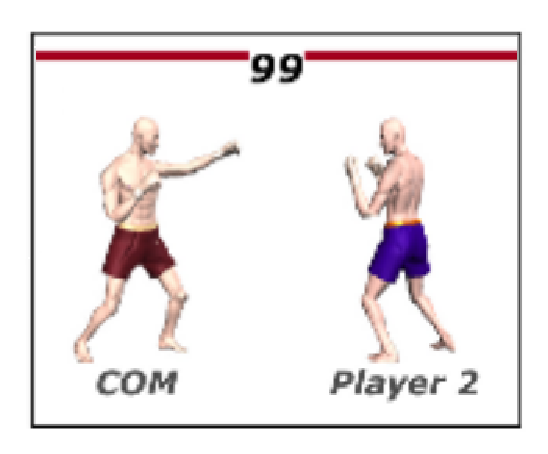
\includegraphics[width=0.5\columnwidth]{chap2/Imagenes/Imitating.eps}
\caption{Ambiente del juego de acci\'on\cite{Nakano2006}.}
\label{fig:imitat}
\end{figure}

En el trabajo desarrollado en la Universidad Tecnol\'ogica de Lanzhou en China
 \cite{Zhang2017},hacen un an\'alisis del comportamiento del soldador experto
 humano utilizando un sistema de inferencia neurodifuso adaptativo (ANFIS,
 por sus siglas en ingl\'es) para su automatizaci\'on, considerando las
 variables
 de los materiales usados y caracterizando la tarea del soldador humano.
 En la figura~\ref{fig:syswelding} se puede apreciar el sistema experimental
  resultante del proyecto mencionado.


\begin{figure}[h]
\centering
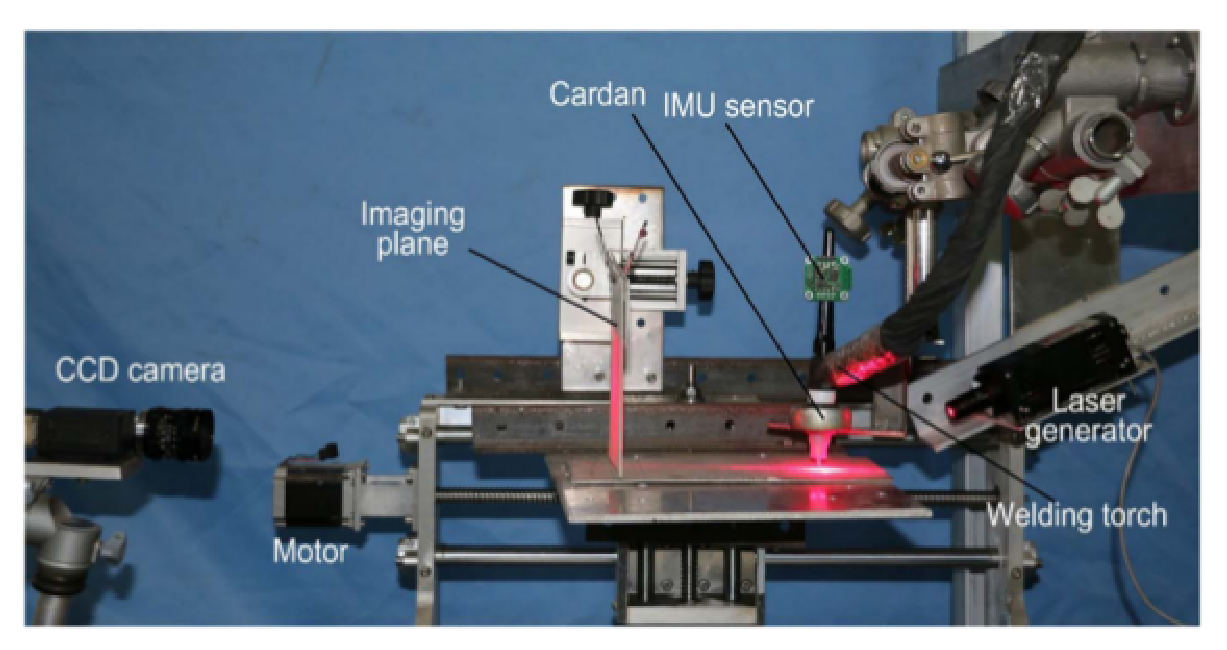
\includegraphics[width=0.8\columnwidth]{chap2/Imagenes/Welding.eps}
\caption{Sistema experimental de la soldadora\cite{Zhang2017}.}
\label{fig:syswelding}
\end{figure} 
 
En el ambiente art\'istico \cite{Nishiguchi2017}, el trabajo desarrollado en
 Jap\'on por la Universidad de artes de Tokyo y la Universidad de Osaka, cuyo
 objetivo era brindar un comportamiento natural humano a un Robot Humanoide.
 Para cumplir esto utilizaron el conocimiento del director de escena Hirata,
 que dada la precisi\'on en sus instrucciones a los actores, facilita la
 traducci\'on de esas \'ordenes a las reglas para el robot humanoide, adem\'as,
 desarrollaron una interfaz de usuario para que el manejo del robot sea m\'as
 sencillo, ayudando a los principiantes, ya que proporcionan menos datos se
 puede obtener buenos resultados. Como se puede observar en la figura
 ~\ref{fig:theatricalrob} el robot llego a desempe\~nar un amigo del
 personaje principal en la obra ``Night on the milky way train''
 (El tren nocturno de la v\'ia l\'actea) en un escenario real.


\begin{figure}[h]
\centering
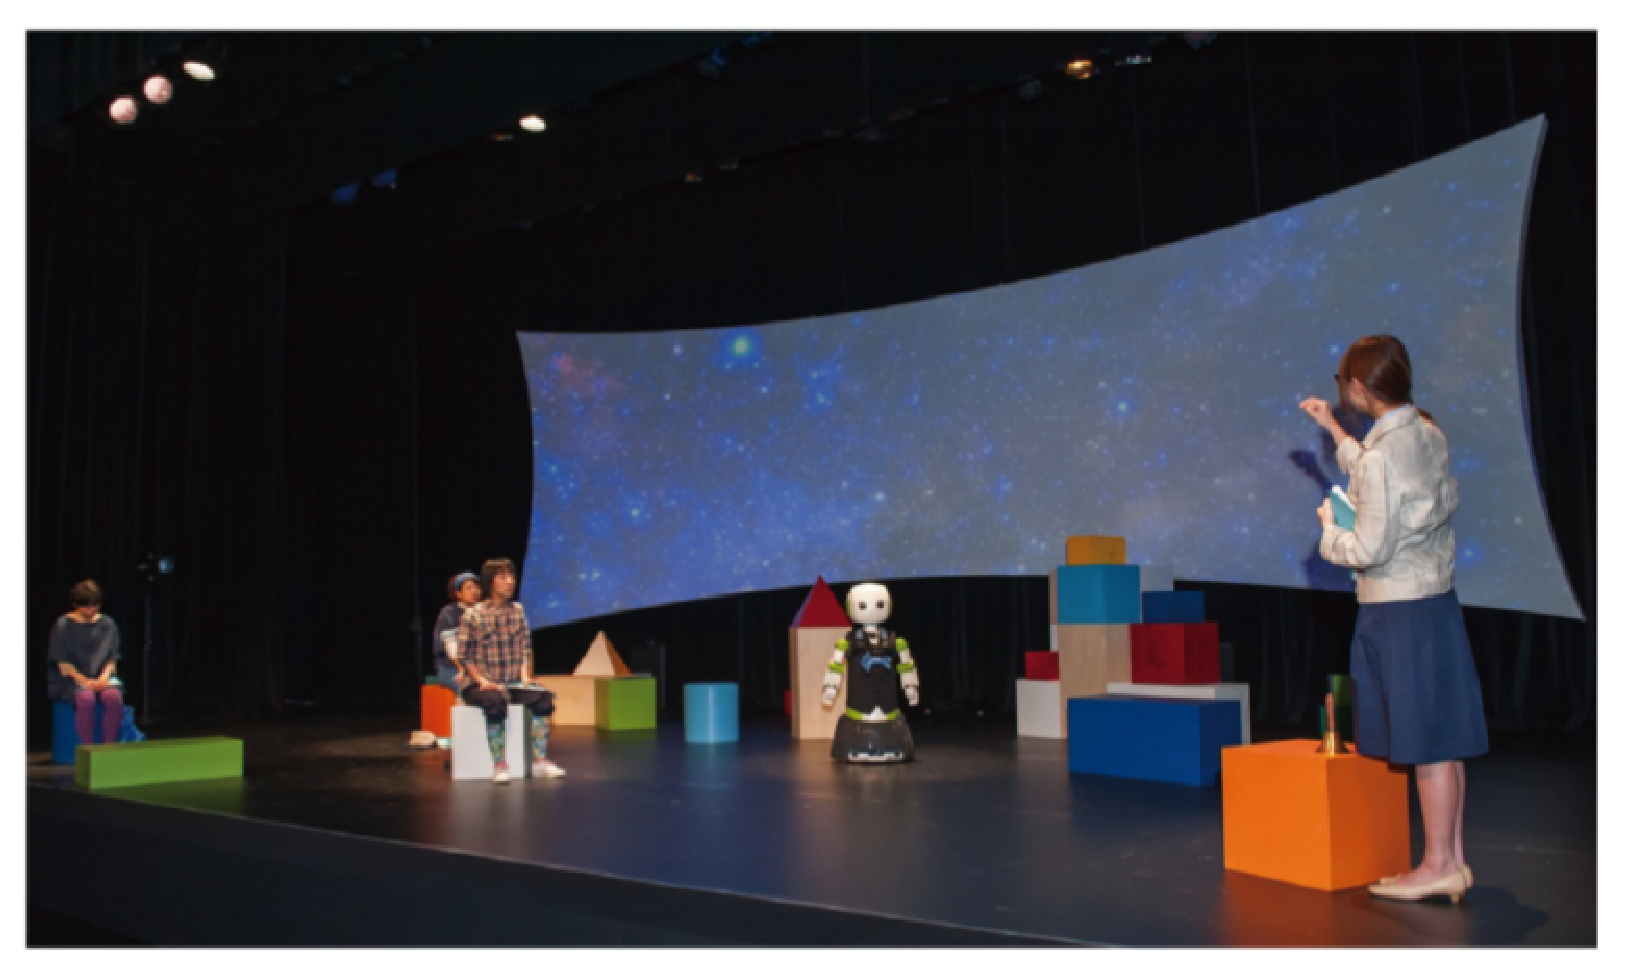
\includegraphics[width=0.8\columnwidth]{chap2/Imagenes/Theatrical.eps}
\caption{Robot humanoide actor en escenario real\cite{Nishiguchi2017}.}
\label{fig:theatricalrob}
\end{figure} 
El trabajo desarrollado por la Universidad de Plymouth, Universidad de
 Lincoln ambas en el Reino Unido y la Universidad de Gante en B\'elgica
 \cite{Senft2016}, realiza un an\'alisis comparativo de su m\'etodo SPARC (Supervised
 Progressively Autonomous Robot Competencies) con el IRL (Interactive
 Reinforcement Learning), estos dos m\'etodos se basan en el aprendizaje 
 autom\'atico de un robot, haciendo que un ser humano con conocimiento del tema
 apruebe la actividad que est\'a realizando o que va a realizar el robot.
 Ambos sistemas fueron probados en un ambiente virtual nombrado ``sophie is
 kitchen''(La cocina de Sofia) cuyo objetivo es hornear un pastel, 
 la figura ~\ref{fig:sparcrob} muestra al robot en la cocina con los materiales
 necesarios para realizar la tarea. 
 
\begin{figure}[h]
\centering
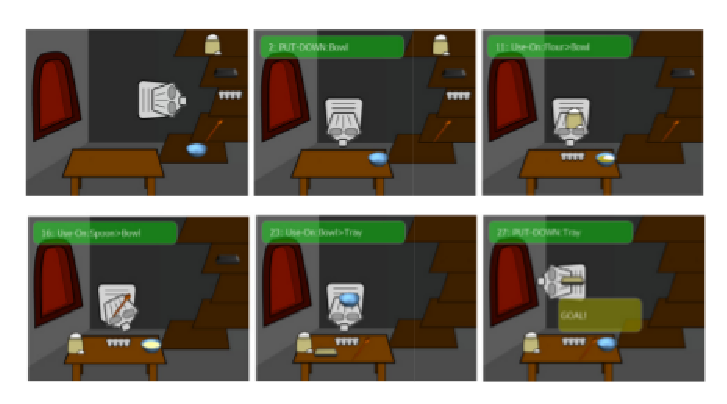
\includegraphics[width=0.8\columnwidth]{chap2/Imagenes/Sparc.eps}
\caption{Robot virtual en ``sophie is kitchen'' (La cocina de Sofia) 
 \cite{Senft2016}.}
\label{fig:sparcrob}
\end{figure}
El trabajo realizado en la Universidad Nacional Chiao Tung y el Instituto
 Polit\'ecnico Kaohsiung ambos en Taiw\'an\cite{Chang1996}, propone un algoritmo
 que imite el comportamiento del aprendizaje humano como una soluci\'on al
 aprendizaje autom\'atico en ambientes imperfectos, por ejemplo, cuando la
 informaci\'on esta incompleta. Este algoritmo demuestra en los experimentos
 realizados ser superior al algoritmo ID3 y PRISM.


\section{Trabajos relacionados}
En \cite{Grasse2010} se presenta el proyecto de la automatizaci\'on de una 
 silla de ruedas VAHM3, en la que se instal\'o un sistema con 3 agentes cuyo
 objetivo es aprender las rutas por las que pasa el usuario de la silla y 
 con apoyo de un mapa topol\'ogico ubicar la silla y ayudar a realizar la ruta
 que el usuario desee, esto usando un algoritmo de condensaci\'on.

 Nuestra propuesta, a diferencia de las anteriores, obtiene, genera, implementa, demuestra, concluye, etc.

% ********** End of chapter **********
